\documentclass[11pt]{article}
\usepackage[a4paper,left=1.5cm,right=1.5cm,top=1.5cm,bottom=1.5cm]{geometry}
\usepackage{fancyhdr}
\renewcommand{\headrulewidth}{1pt}
\fancyhead[C]{\textbf{[LINMA1170] SVD et conditionnement}}
\fancyhead[L]{Novembre 2018}
\fancyhead[R]{Gilles Peiffer [24321600]}

\usepackage[T1]{fontenc}
\usepackage[utf8]{inputenc}
\usepackage[french]{babel}
\usepackage{graphicx}
\usepackage{subcaption}
\usepackage{mathtools,amssymb}
\usepackage[binary-units=true,separate-uncertainty = true,multi-part-units=single]{siunitx}
\usepackage{float}
\usepackage[linktoc=all]{hyperref}
\hypersetup{breaklinks=true}
\setlength{\parindent}{0cm}
\setlength{\parskip}{1ex plus 0.5ex minus 0.2ex}
\newcommand{\hsp}{\hspace{20pt}}
\newcommand{\HRule}{\rule{\linewidth}{0.5mm}}
\graphicspath{{img/}}
\usepackage{caption}
\usepackage{textcomp}
\usepackage{array}
\usepackage{color}
\usepackage{tabularx,booktabs}
\usepackage{titlesec}
\titlespacing{\section}{0pt}{\parskip}{-\parskip}
\titlespacing{\subsection}{0pt}{\parskip}{-\parskip}
\titlespacing{\subsubsection}{0pt}{\parskip}{-\parskip}
\pagestyle{fancy}
\DeclarePairedDelimiterX{\norm}[1]{\lVert}{\rVert}{#1}

\begin{document}
\section{Paramètres influençant le conditionnement de $A$}
\label{param}
\subsection{Largeur de l'entrefer}
Moins l'entrefer est large, plus le maillage doit être raffiné à cet endroit.
Nous remarquons donc que pour des entrefers de petite taille,
le conditionnement de la matrice augmente rapidement (figure~\ref{fig:gapcond}).
Si nous appelons $e$ la taille de l'entrefer, on peut écrire
\[
\kappa(A) \sim \alpha + \frac{\beta}{e}\,, \quad \alpha, \beta \in \mathbb{R}\,.
\]

Le spectre reste distribué de façon semblable peu importe la taille de l'entrefer,
mais plus celui-ci est grand, moins il y a de valeurs singulières, comme montré sur la figure~\ref{fig:gapspec}.

Lorsque nous commentons la ligne \texttt{lc3=D/2.*R} et la remplaçons par \texttt{lc3=E/2.*R}, nous augmentons en fait la taille de l'entrefer.
L'effet sur le maillage est montré à la figure~\ref{fig:mesh}.

\subsection{Perméabilité relative du noyau magnétique}
Plus la perméabilité relative du noyau magnétique augmente,
plus le conditionnement de $A$ augmente aussi, selon une loi approximativement logarithmique (voir figure~\ref{fig:mucond}). On écrit (en notant $\mu_{\mathrm{r}}$ la perméabilité)
\[
\kappa(A) \sim \gamma + \delta \log(\mu_{\mathrm{r}} + \varepsilon)\,, \quad \gamma, \delta, \varepsilon \in \mathbb{R}\,. 
\]

Le spectre change uniquement pour les valeurs singulières les plus petites,
et celles-ci deviennent encore plus basses, comme montré sur la figure~\ref{fig:muspec}.

\subsection{Courant injecté dans la bobine}
Le courant injecté dans la bobine ne change en rien le maillage,
et n'a donc aucun effet ni sur le conditionnement de la matrice $A$,
ni sur son spectre de valeurs singulières,
comme montré aux figures~\ref{fig:jcond} et~\ref{fig:jspec}.

\subsection{Raffinement du maillage}
Afin de voir l'effet du raffinement du maillage sur le conditionnement de la matrice $A$, nous avons joué sur le paramètre \texttt{clscale} de \texttt{ccore.py}.
Plus celui-ci est petit, plus le maillage est fin.
Le conditionnement de $A$ diminue de façon linéaire plus \texttt{clscale} augmente, mais augmente soudainement pour la valeur de $34$ (voir figure~\ref{fig:clscalecond}).
Cela est dû à l'algorithme de maillage, qui calcule pour cette valeur de \texttt{clscale} des éléments très plats (mauvais pour le conditionnement).
On écrit donc en général (en notant \texttt{clscale} par $c$)
\[
\kappa(A) \sim \left\{ \begin{array}{ll}
\zeta + \eta c & \textnormal{si $c < 34$}\,,\\
\theta + \iota c & \textnormal{sinon,}
\end{array}\right. \quad \zeta, \eta, \theta, \iota \in \mathbb{R}\,.
\]

Le spectre des valeurs singulières a toujours la même forme,
mais est ``compressé'' lorsque le paramètre \texttt{clscale} augmente, comme montré sur la figure~\ref{fig:clscalespec}.

\section{Approximation de rang faible}
\label{approx}
Nous cherchons à approximer la matrice $A \in \mathbb{R}^{m \times n}$ de rang $r$ par une somme de $\nu$ matrices de rang $1$ comme suit:
\(
A_{\nu} = \sum_{j=1}^{\nu} \sigma_{j} u_{j} v^*_{j}\,. 
\) 
Par le Théorème~5.8 pp. 35--36 dans le livre de référence,
il est possible de démontrer que cette somme partielle
capture l'énergie maximale possible de $A$,
et ce autant pour la $2$-norme matricielle (avec laquelle nous travaillons)
que pour la norme de Frobenius.
On définit alors l'erreur $e_{\nu}$ comme
\(
e_{\nu} = \frac{\norm{A - A_{\nu}}_2}{\norm{A}_2}\,.
\)

\subsection{Influence du premier terme}
Plus le système devient grand, moins le premier terme représente une grande partie de l'énergie totale, comme montré sur la figure~\ref{fig:clscalefirst}.
La relation est approximativement linéaire.

\subsection{Nombre de termes requis pour obtenir une précision donnée}
Autant pour une erreur inférieure à $\SI{10}{\percent}$ qu'à $\SI{1}{\percent}$, on observe une relation inversement proportionelle (voir figures~\ref{fig:clscale10} et~\ref{fig:clscale1}).

\subsection{Influence du conditionnement}
L'influence du conditionnement est donc difficile à définir, car en utilisant les données de la question~\ref{param}, on voit que le conditionnement effectue un saut en fonction de \texttt{clscale} (figure~\ref{fig:clscalecond} autour de la valeur $34$), alors que ce n'est pas le cas pour le pourcentage d'énergie contenu dans le premier terme, ni pour le nombre de termes requis pour borner l'énergie.

\appendix
\section{Appendice: figures}
\begin{figure}[H]
	\centering
	\begin{subfigure}[t]{0.24\textwidth}
		\centering
		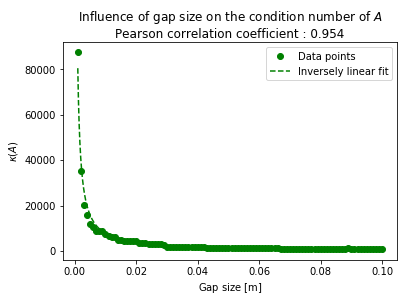
\includegraphics[width=\linewidth]{gapcond.png}
		\caption{Influence de la taille de l'entrefer sur le  conditionnement de $A$.}
		\label{fig:gapcond}
	\end{subfigure}\hfill
	\begin{subfigure}[t]{0.24\textwidth}
		\centering
		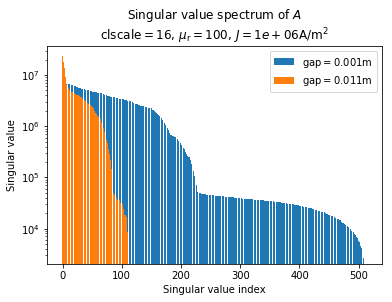
\includegraphics[width=\linewidth]{gapspec.png}
		\caption{Influence de la taille de l'entrefer sur le spectre des valeurs singulières de $A$.}
		\label{fig:gapspec}
	\end{subfigure}\hfill
	\begin{subfigure}[t]{0.24\textwidth}
		\centering
		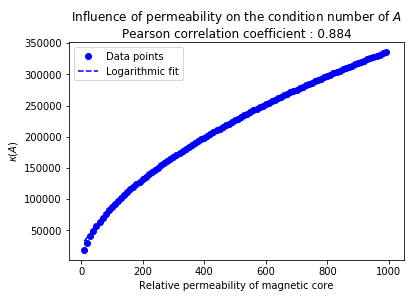
\includegraphics[width=\linewidth]{mucond.png}
		\caption{Influence de la perméabilité relative $\mu_{\textnormal{r}}$ sur le conditionnement de $A$.}
		\label{fig:mucond}
	\end{subfigure}\hfill
	\begin{subfigure}[t]{0.24\textwidth}
		\centering
		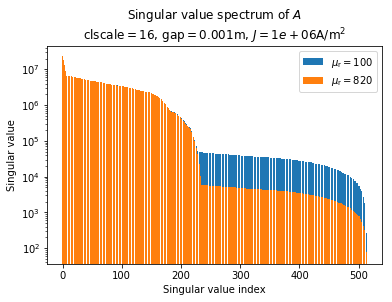
\includegraphics[width=\linewidth]{muspec.png}
		\caption{Influence de la perméabilité relative $\mu_{\textnormal{r}}$ sur le spectre des valeurs singulières de $A$.}
		\label{fig:muspec}
	\end{subfigure}
	\begin{subfigure}[t]{0.24\textwidth}
		\centering
		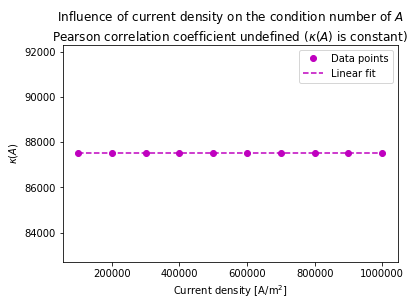
\includegraphics[width=\linewidth]{jcond.png}
		\caption{Influence de la densité de courant sur le conditionnement de la matrice $A$.}
		\label{fig:jcond}
	\end{subfigure}\hfill
	\begin{subfigure}[t]{0.24\textwidth}
		\centering
		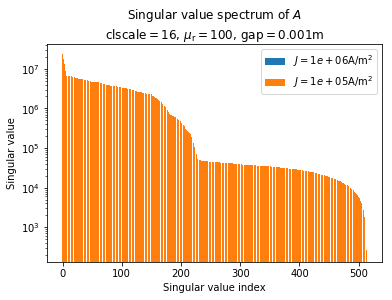
\includegraphics[width=\linewidth]{jspec.png}
		\caption{Influence de la densité de courant sur le spectre des valeurs singulières de $A$.}
		\label{fig:jspec}
	\end{subfigure}\hfill
	\begin{subfigure}[t]{0.24\textwidth}
		\centering
		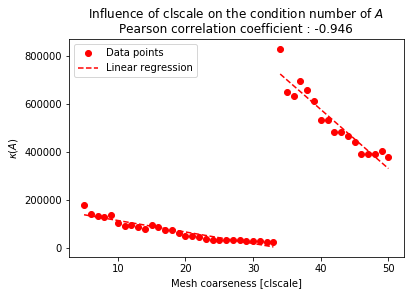
\includegraphics[width=\linewidth]{clscalecond.png}
		\caption{Influence du raffinement du maillage sur le conditionnement de $A$.}
		\label{fig:clscalecond}
	\end{subfigure}\hfill
	\begin{subfigure}[t]{0.24\textwidth}
		\centering
		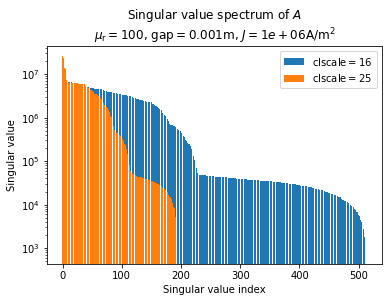
\includegraphics[width=\linewidth]{clscalespec.png}
		\caption{Influence du raffinement du maillage sur le spectre des valeurs singulières de $A$.}
		\label{fig:clscalespec}
	\end{subfigure}
	\caption{Différents graphes pertinents pour l'analyse de la section~\ref{param}.
	Les coefficients de correlation sont toujours calculés par rapport au \emph{curve fit} proposé.}
	\label{fig:figsec1}
\end{figure}

\begin{figure}[H]
	\centering
	\begin{subfigure}{0.25\textwidth}
		\centering
		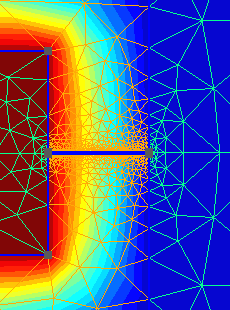
\includegraphics[width=\linewidth]{mesh1.png}
		\caption{Avec \texttt{lc3=D/2.*R}.}
		\label{fig:mesh1}
	\end{subfigure}\hspace{3cm}
	\begin{subfigure}{0.25\textwidth}
		\centering
		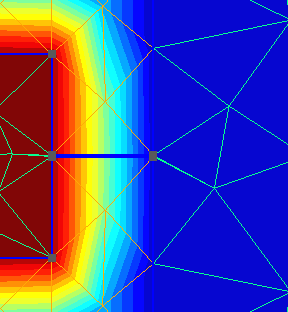
\includegraphics[width=\linewidth]{mesh2.png}
		\caption{Avec \texttt{lc3=E/2.*R}.}
		\label{fig:mesh2}
	\end{subfigure}
	\caption{Comparaison des maillages en changeant une ligne de code.}
	\label{fig:mesh}
\end{figure}

\begin{figure}[H]
	\centering
	\begin{subfigure}[t]{0.32\textwidth}
		\centering
		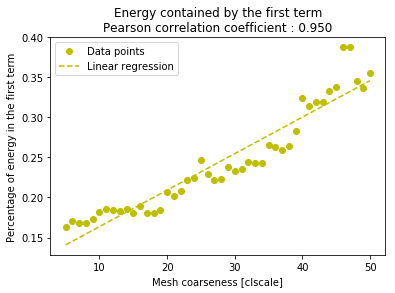
\includegraphics[width=\linewidth]{clscalefirst.png}
		\caption{Pourcentage de l'énergie totale contenue dans le premier terme de la somme décroissant.}
		\label{fig:clscalefirst}
	\end{subfigure}\hfill
	\begin{subfigure}[t]{0.32\textwidth}
		\centering
		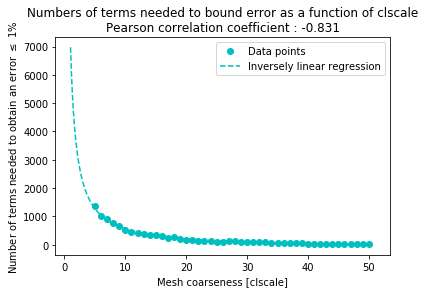
\includegraphics[width=\linewidth]{clscale1.png}
		\caption{Nombre de termes requis pour obtenir une erreur $e_{\nu} \le \SI{1}{\percent}$.}
		\label{fig:clscale1}
	\end{subfigure}\hfill
	\begin{subfigure}[t]{0.32\textwidth}
		\centering
		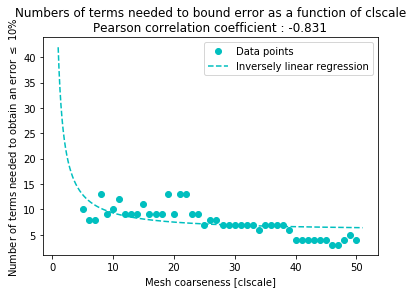
\includegraphics[width=\linewidth]{clscale10.png}
		\caption{Nombre de termes requis pour obtenir une erreur $e_{\nu} \le \SI{10}{\percent}$.}
		\label{fig:clscale10}
	\end{subfigure}
	\caption{Différents graphes pertinents pour l'analyse de la section~\ref{approx}.
	Les coefficients de correlation sont toujours calculés par rapport au \emph{curve fit} proposé.}
	\label{fig:figsec2}
\end{figure}
\end{document}